\chapter{Problemas \textsl{NP}-completos y \textsl{NP}-duros}

Aunque el término de computación ha existido por cientos 
de años, no fue sino hasta que su significado cambió de \textit{una persona que 
realiza cálculos siguiendo ciertas reglas} a lo que se le conoce hoy en día, 
que hizo necesario generar una clasificación de problemas a calcular. 
Se mostrará que la clasificación por clases de problemas fue una consecuencia 
natural temprana y se enuncian las definiciones de dichas clases.

\section{Historia y definición}
\label{sec:np-def}

A principios del siglo XX, en agosto de 1900 se llevó acabo el segundo
congreso internacional de matemáticas en París, Francia.
Motivado por el congreso y la llegada de un nuevo siglo, el matemático
David Hilbert planteó un conjunto de veintitrés problemas de lo que él llamó
``el futuro problema de las matemáticas''.
Para 1902, Hilbert mantenía un optimismo sobre la resolución de sus problemas,
diciendo: \textit{For in mathematics there is no ignorabimus!} [Para las matemáticas
no existe el \emph{ignorabimus}\footnote{La palabra \textit{ignorabimus} a la que
Hilbert hace referencia, tiene origen en un latinismo que dice
\textit{Ignoramus et ignorabimus} y significa  ``desconocemos y
desconoceremos''.}]~\cite{Grattan-Guinness}. Veintiocho años más tarde y aunque
Hilbert no lo incluyó en su lista de veintitrés problema originales, enunció
otro para la comunidad matemática: crear un algoritmo que tome como entrada
un predicado (con un número finito de axiomas y enunciados) y regrese como
resultado ``Sí'' o ``No'' si es universalmente válido. Este problema es conocido
como el \textit{Entscheidungsproblem} o el problema de
decisión~\cite{hilbert1950principles}. En otras palabras, el problema de
decisión consiste en averiguar si existe un algoritmo genérico que decida
si un problema matemático tiene o no demostración.

En el año 1936, el matemático Alan Turing publicó un artículo que
revolucionó e impactó al mundo y a las matemáticas; de nombre \textit{
Sobre los números computables, con una aplicación al Entscheidungsproblem}
\footnote{El título original es \textit{On computable numbers, with an
application to the Entscheidungsproblem}.}; en este trabajo Turing
definió \textit{una máquina de cómputo} después denominada como \textit{
máquina de Turing} y una \textit{máquina de cómputo universal}. De forma
paralela y del otro lado del océano Atlántico, Alonso Church publicó su trabajo
llamado en inglés \textit{An Unsolvable Problem of Elementary Number Theory},
donde de manera independiente pero casi simultanea a Turing, trabajó sobre
el \emph{Entscheidungsproblem} usando el modelo llamado \textit{cálculo
lambda}~\cite{church1935unsolvable}. Años más tarde, Alan Turing y Alonso Church
trabajarían juntos para formular la equivalencia de sus modelos~\cite{sep-church-turing}.

La máquina de Turing o MT es un modelo matemático de una computadora hipotética
la cual usa un conjunto predefinido de reglas para determinar el resultado de
un conjunto de variables de entrada\footnote{\cite{gurovich2015introduccion}
define formalmente a una máquina de Turing como un 7-tuplo $M=(Q,\Sigma, \Gamma,
\delta, q_{0}, \square,F)$.}. La máquina de cómputo universal o \textit{Máquina
de Turing universal} es una máquina que puede computar cualquier secuencia
computable dada una descripción de una máquina $M$. La máquina universal $U(M)$
puede realizar exactamente los mismos cómputos de $M$.

En ese mismo artículo Alan Turing, además de plantear el \emph{Entscheidungsproblem}
usando su máquina de Turing y la máquina universal para demostrar que el
planteamiento de Hilbert era falso, Turing usa el proceso de diagonalización para
mostrar que no se puede construir un proceso que tome la descripción general de
una MT y nos diga si es libre de ciclos (\textit{circle-free}) o terminará su
ejecución; este problema se le conoce como \textit{El problema del paro} o
\textit{The Halting Problem}. Con estos resultados Alan Turing crea una primera
clasificación de problemas para las MT: los problemas computables y los no
computables~\cite{Turing1936}.

Posterior a esta primera clasificación, hubo la necesidad de seguir dividiendo
los problemas desde el punto de vista de otra restricción que presentan las MT.
Desde el inicio del uso de las primeras computadoras electrónicas, se
descubrió que el modelo básico de las máquinas de Turing fallan al considerar
la cantidad de tiempo o memoria que necesita una computadora real, un
problema crítico en la actualidad pero más aún en aquellos primeros días de
la computación moderna. La idea clave para medir el tiempo y el espacio en función
de la longitud de la entrada llegó a principio de la década de los sesentas,
por Juris Hartmanis y Richard Stearns cuyo artículo \textit{Sobre la complejidad
computacional de los algoritmos}\footnote{\textit{On the Computational
Complexity of Algorithms} es el título original.} sentó las bases de lo que
se conoce como complejidad computacional~\cite{Hartmanis1965}.

Al principio de la teoría, las investigaciones giraban en torno a
sólo tratar de entender éstas nuevas formas de medición y cómo se
relacionaban entre ellas. En los sesentas también se menciona por primera vez el
término de \textit{clases de complejidad} y se genera un concepto de eficiencia
computacional al medir el tamaño de la entrada con polinomios~\cite{Fortnow2002}.

Para entender las distintas \textit{clases de complejidad} y antes de enunciar
las definiciones formales de \textsl{P}, \textsl{NP}, \textsl{NP}-completo y
\textsl{NP}-duro, se enunciará un ejemplo que puede ser útil para entender la
dificultad de los cálculos que realizan las máquinas para encontrar soluciones
de algoritmos no triviales: suponer que existe un gran grupo de estudiantes
en los que se necesita que trabajen en equipo para un proyecto, se sabe qué
estudiantes son compatibles entre sí y se desea colocar a los estudiantes en
equipos compatibles. Es deseable que los equipos sean con la menor cantidad de
integrantes, dos de ser posible y así todos los estudiantes realicen alguna
parte del proyecto. Una forma de encontrar la solución sería calcular todos los
posibles equipos y descartar los que tienen personas que no se lleven 
bien entre sí; pero para una muestra de 40 estudiantes, podrían existir más de
300 mil trillones de posibles equipos (las combinaciones que forman particiones
del conjunto potencia de estudiantes). Este programa se le llama \textit{Mínimo
  apareamiento maximal}~\cite{10.1007/978-3-540-79228-4_32}.  En 1965, Jack
Edmonds describió un algoritmo eficiente para resolver el problema de
emparejamiento y sugirió una definición formal de \textit{eficiencia
  computacional} \cite{Mathematics}. La clase de problemas con soluciones
eficientes sería luego renombrada como la clase \textsl{P}\footnote{Viene del
  inglés \textit{Polynomial Time} que significa tiempo polinomial.}.

Para muchos problemas parecidos y relacionados no se conoce un algoritmo
eficiente que pueda resolverlos: regresando al ejemplo de los estudiantes, ¿cuál
sería el algoritmo si ahora se hacen grupos de al menos tres? (partición de triángulos)
¿Qué pasa si se quiere sentar a los estudiantes en una mesa redonda sin que sean
vecinos de algún alumno incompatible? (Ciclo Hamiltoniano) ¿Y si se ponen a los
estudiantes en tres grupos y que cada estudiante se encuentre en un grupo sólo
con personas compatibles? (3-coloración).  Todos estos problemas tienen en común
que dada una posible solución, se puede corroborar que sea correcta en un tiempo
eficiente.  La colección de problemas que tienen soluciones verificables en
tiempo eficiente es conocida como la clase \textsl{NP}\footnote{Viene del inglés
  \textit{ Nondeterministic Polynomial-Time}.}.

En 1971 Stephen Cook y Leonid Levin hicieron la demostración que lleva sus
apellidos, en la que prueban que cualquier problema \textsl{NP} puede
ser \textit{reducido} en tiempo polinomial por una máquina de Turing
determinista a un problema en específico. El concepto
(mas no el término) de \textsl{NP}-completez fue presentado por primera
vez en~\cite{Cook}.
En la demostración del trabajo Cook-Levin, los autores muestran el
\textit{Problema de satisfacibilidad booleana}, también conocido como
\texttt{\textbf{SAT}}, como el primer problema \textsl{NP}-completo.
\texttt{SAT} consiste en determinar si una fórmula booleana es o
no satisfacible; en otras palabras, si existe
alguna asignación de valores para sus variables que haga a la expresión
verdadera.

Formalmente se dice que si $\varphi$ es una fórmula booleana con
variables $u_{1}, u_{2}, \ldots, u_{n}$ y $z \in \{0,1\}^{n}$, entonces
$\varphi(z)$ denota el valor de $\varphi$ cuando a las variables de $\varphi$
le son asignados los valores de $z$. Una fórmula $\varphi$ es satisfacible si
existe una asignación $z$ tal que $\varphi(z)$ sea \texttt{TRUE}. Si no existe
$z$ para $\varphi(z) = \texttt{TRUE}$, se dice que $\varphi$ es
insatisfacible~\cite{arora2009computational}. Sólo un año después de la
demostración, en su artículo \textit{Reducibility Among Combinatorial Problems} el computólogo
Richard M. Karp, usó las conclusiones del trabajo para definir 21 problemas
\textsl{NP}-completos adicionales~\cite{Karp1972}.

Para poder enunciar las definiciones formales de las clases \textsl{P} y \textsl{NP},
se necesita conocer al menos tres definiciones relacionadas previamente:
lenguaje decidible, la clase \texttt{DTIME} y reductibilidad. Las siguientes
siete definiciones formales son tomadas de~\cite{arora2009computational}:

\begin{enumerate}
 \item
  Se dice que una máquina decide un lenguaje $L \subseteq \{0, 1\}^{*}$ si
 calcula la función $f_{L}:\{0,1\}^{*} \longrightarrow \{0,1\}$, donde
 $f_{L} (x) = 1 \Leftrightarrow x \in L$.

 \item
  Sea $T: \mathbb{N} \longrightarrow \mathbb{N}$
 alguna función. Un lenguaje \textsl{L} es elemento de \texttt{DTIME}$(T(n))$ si y sólo
 si existe alguna máquina de Turing que corra en tiempo $c \cdot T(n)$ para alguna
 constante $c > 0$ y que decida $L$.

 \item
Un lenguaje $L \subseteq \{0,1\}^{*}$ es polinonialmente \textbf{reducible} a
un lenguaje $L' \subseteq \{0,1\}^{*}$ (también llamado
\textit{Karp reducible}), denotado por $L \leq_{p} L'$, si existe una
función computable en tiempo polinomial
$f : \{0,1\}^{*} \longrightarrow \{0,1\}^{*}$ tal que para cada
$x \in \{0,1\}^{*}$, $x \in L$ si y sólo si $f(x) \in L'$.
\end{enumerate}

\noindent
Dada las definiciones anteriores y el ejemplo mencionado, se pueden enunciar las
definiciones formales de las clases \textsl{P} y \textsl{NP} y el resto de las
clases de complejidad:

\begin{enumerate}
  \setcounter{enumi}{3}

\item Se define a la clase \textsl{P} como
  $\textsl{P} = \cup_{c \geq 1} ~ \texttt{DTIME}(n^{c})$.

\item Un lenguaje $L \subseteq \{0, 1\}^{*}$ está en \textsl{NP} si existe un
  polinomio $p: \mathbb{N} \longrightarrow \mathbb{N}$ y una máquina de Turing
  que se ejecute en tiempo polinomial $M$ (llamada la verificadora de $L$) tal
  que para cada $x \in \{0,1\}^{*}$,

  \begin{displaymath}
    x \in L \Leftrightarrow \exists u \in \{0,1\}^{p(|x|)},~
    \textrm{tal que} ~ M(x,u) = 1.
  \end{displaymath}

\item Se dice que $L'$ es \textsl{NP}-duro o \textsl{NP}-duro si
  $L \leq_{p} L'$ para cada $L \in \textsl{NP} $.

\item Se dice que $L'$ es \textsl{NP}-completo si $L'$ es \textsl{NP}-duro y
  $L' \in \textsl{NP}$.

\end{enumerate}




\section{3-Partición}
\label{sec:3-particion}

El problema de \texttt{3-PARTITION} o 3-Partición es un problema \textsl{NP}-completo,
el cual enuncia que dado un conjunto finito $\mathcal{A}$ de $3m$ elementos,
una cota $b \in \mathds{Z}^{+}$ y una ``medida''\footnote{El autor usa la
palabra \textit{``size''} como alternativa a una mejor palabra para la función.}
$s(a) \in \mathds{Z}^{+}$ con $a \in \mathcal{A}$, tal que
satisfaga que $b/4 < s(a) < b/2$ y que $\sum_{a \in \mathcal{A}} s(a) = m \cdot b$,
¿puede $\mathcal{A}$ ser particionado en $m$ conjuntos disjuntos $S_{1}, S_{2},
S_{3}, \ldots , S_{m}$ tal que para cada $1 \leq i \leq m $, $\sum_{a \in S_{i}}
s(a)=b$? En otras palabras, dado un conjunto de $N$ elementos,
¿puede encontrarse una partición de $N/3$ subconjuntos tal que la suma de los
elementos de cada uno debe ser la misma y la cardinalidad de cada subconjunto
debe ser tres?

La definición de 3-partición (o \texttt{3-PARTITION}), junto con la demostración
de su \mbox{\textsl{NP}-completez} apareció en el año de 1979 y es visto como
un problema de decisión~\cite{Garey:1990:CIG:574848}. Para la demostración de la
\textsl{NP}-completez del problema se usa una reducción del problema de la
4-partición, el cual es \textsl{NP}-completo y previamente demostrado a partir
del problema general de la partición
(\cref{fig:secuenciaNP}). \texttt{3-PARTITION} es un problema de los llamados
\textit{totalmente o fuertemente \textsl{NP}-completos}, esto quiere decir que
sigue siendo \textsl{NP}-completo incluso cuando los enteros (o elementos) de
$\mathcal{A}$ están acotados por un polinomio en $N$.

\begin{figure}[h]
\centering
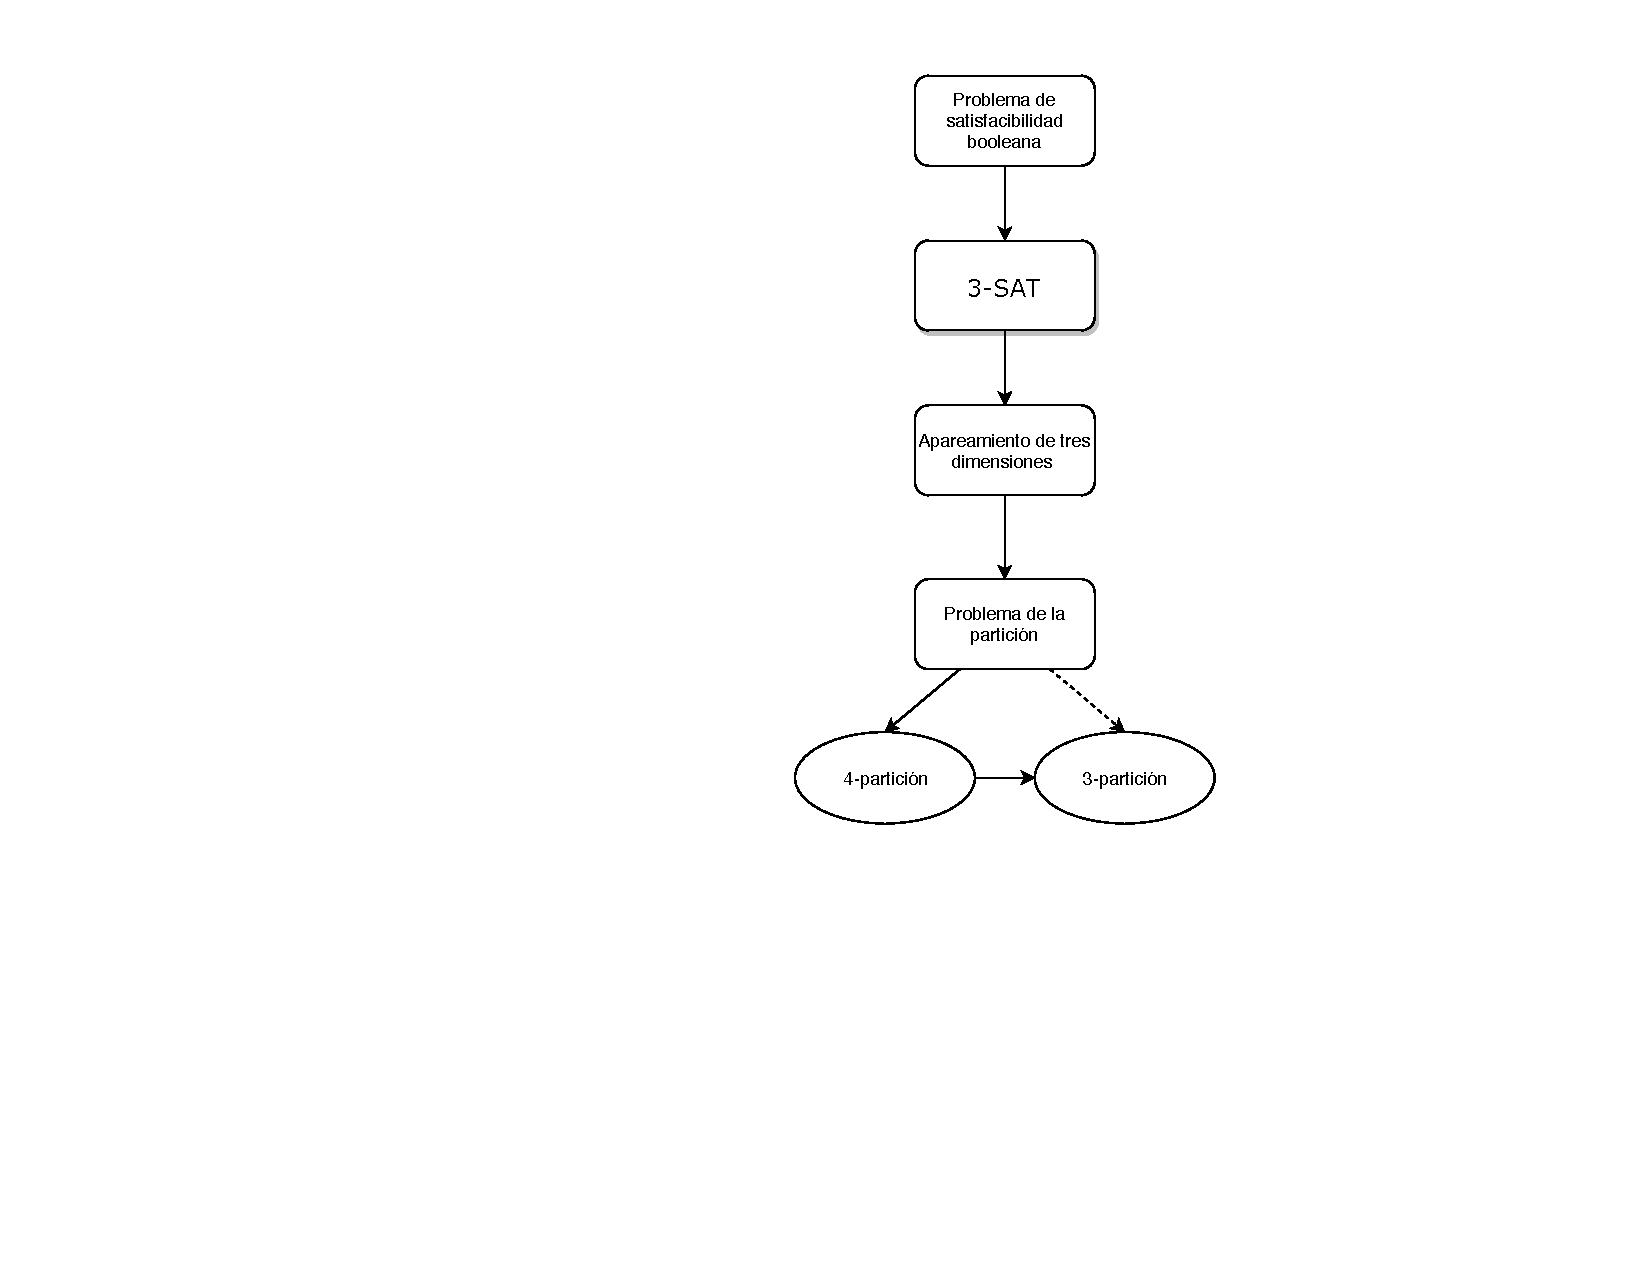
\includegraphics[width=.45\textwidth,keepaspectratio,trim={12cm 6cm 7cm 0cm}]{./images/2_2_1.pdf}
\caption{Diagrama de la secuencia de las transformaciones usadas para
probar que 3-partición es \textsl{NP}-completo.}
\label{fig:secuenciaNP}
\end{figure}

Este trabajo se encuentra íntimamente relacionado al problema y clasificación de
la 3-partición debido al resultado de la \textit{fuerte \textsl{NP}-completez};
esta propiedad será de utilidad cuando se tenga que explicar la simplificación de
una representación unaria del problema a implementar, como se discutirá en el
\cref{chap:cuatro}. Varias afirmaciones posteriores parten del hecho de que
hay una reducción de la 3-partición por lo que no se sabe si existe un método de
resolución eficiente al problema presentado en esta tesis.

%%% Local Variables:
%%% mode: latex
%%% TeX-master: "../main"
%%% End:
